\documentclass[a4paper,11pt]{article}
\usepackage{amsmath,amsthm,amsfonts,amssymb,amscd,amstext,vmargin,graphics,graphicx,tabularx,multicol} 
\usepackage[francais]{babel}
\usepackage[utf8]{inputenc}  
\usepackage[T1]{fontenc} 
\usepackage{pstricks-add,tikz,tkz-tab,variations}
\usepackage[autolanguage,np]{numprint} 
\usepackage{calc}

\setmarginsrb{1.5cm}{0.5cm}{1cm}{0.5cm}{0cm}{0cm}{0cm}{0cm} %Gauche, haut, droite, haut
\newcounter{numexo}
\newcommand{\exo}[1]{\stepcounter{numexo}\noindent{\bf Exercice~\thenumexo} : }
\reversemarginpar

\newcommand{\bmul}[1]{\begin{multicols}{#1}}
\newcommand{\emul}{\end{multicols}}

\newcounter{enumtabi}
\newcounter{enumtaba}
\newcommand{\q}{\stepcounter{enumtabi} \theenumtabi.  }
\newcommand{\qa}{\stepcounter{enumtaba} (\alph{enumtaba}) }
\newcommand{\initq}{\setcounter{enumtabi}{0}}
\newcommand{\initqa}{\setcounter{enumtaba}{0}}

\newcommand{\be}{\begin{enumerate}}
\newcommand{\ee}{\end{enumerate}}
\newcommand{\bi}{\begin{itemize}}
\newcommand{\ei}{\end{itemize}}
\newcommand{\bp}{\begin{pspicture*}}
\newcommand{\ep}{\end{pspicture*}}
\newcommand{\bt}{\begin{tabular}}
\newcommand{\et}{\end{tabular}}
\renewcommand{\tabularxcolumn}[1]{>{\centering}m{#1}} %(colonne m{} centrée, au lieu de p par défault) 
\newcommand{\tnl}{\tabularnewline}

\newcommand{\trait}{\noindent \rule{\linewidth}{0.2mm}}
\newcommand{\hs}[1]{\hspace{#1}}
\newcommand{\vs}[1]{\vspace{#1}}

\newcommand{\N}{\mathbb{N}}
\newcommand{\Z}{\mathbb{Z}}
\newcommand{\R}{\mathbb{R}}
\newcommand{\C}{\mathbb{C}}
\newcommand{\Dcal}{\mathcal{D}}
\newcommand{\Ccal}{\mathcal{C}}
\newcommand{\mc}{\mathcal}

\newcommand{\vect}[1]{\overrightarrow{#1}}
\newcommand{\ds}{\displaystyle}
\newcommand{\eq}{\quad \Leftrightarrow \quad}
\newcommand{\vecti}{\vec{\imath}}
\newcommand{\vectj}{\vec{\jmath}}
\newcommand{\Oij}{(O;\vec{\imath}, \vec{\jmath})}
\newcommand{\OIJ}{(O;I,J)}


\newcommand{\reponse}[1][1]{%
\multido{}{#1}{\makebox[\linewidth]{\rule[0pt]{0pt}{20pt}\dotfill}
}}

\newcommand{\titre}[5] 
% #1: titre #2: haut gauche #3: bas gauche #4: haut droite #5: bas droite
{
\noindent #2 \hfill #4 \\
#3 \hfill #5

\vspace{-1.6cm}

\begin{center}\rule{6cm}{0.5mm}\end{center}
\vspace{0.2cm}
\begin{center}{\large{\textbf{#1}}}\end{center}
\begin{center}\rule{6cm}{0.5mm}\end{center}
}



\begin{document}
\pagestyle{empty}
\titre{Séance d'AP  : les puissances}{}{}{4ème}{}


\vspace*{0.2cm}

\setlength{\fboxrule}{2pt}
\begin{flushleft}
\framebox{\begin{minipage}{\linewidth}

\vspace*{0.5cm}

\underline{\textbf{Rappels de cours}}\\

\textbf{Définition 1:} \hspace*{1cm} $a^{n} = \underbrace{a \times ... \times a}_{n fois}$  \hspace*{1.5cm}  $a^{-n} = \dfrac{1}{\underbrace{a \times ... \times a}_{n fois}}$ \\

\textbf{Remarques :} \hspace*{1cm}  $a^{1} = a$ \hspace*{1.5cm} $a^{0} = 1$\\

\textbf{Propriétés :} \hspace*{0.2cm}  $a^{n} \times a^{m} =a^{n+m}$ \hspace*{0.5cm} $\dfrac{a^{n}}{a^{m}}=a^{n-m}$ \hspace*{0.5cm} $ (a^{n})^{m} = a^{n\times m}$ \hspace*{1cm} $a^{n}\times b^{n} = (a\times b)^{n} $ \hspace*{0.5cm} $\dfrac{a^{m}}{b^{m}} = \left(\dfrac{a}{b} \right)^{m}$\\
\vspace*{0.5cm}

\textbf{Définition 2 :}\textbf{ L'écriture scientifique }d'un nombre décimal est l'unique écriture de ce nombre sous la forme $a \times 10^{n}$, où:
\bi
\item $a$ est un nombre décimal compris entre 1 et 10, 10 étant exclu ;
\item $n$ est un nombre entier relatif (positif ou négatif).\\
\ei
\vspace*{0.2cm}

\textbf{Exemples :}  $2,145 \times 10^{5}$ est l'écriture scientifique du nombre 214 500\\
 \hspace*{ 1.8cm}               $1,25 \times 10^{-2}$  est l'écriture scientifique du nombre 0, 0125


\vspace*{0.5cm}
\end{minipage}}
\end{flushleft}

\vspace*{1cm}


\exo \\
Sept  voitures  transportent  chacune  sept  personnes  qui  possèdent  chacune  un  sac  avec  sept  poches.  Dans chaque poche se trouve sept enveloppes contenant chacune sept photographies.\\
Quel est le nombre total de photographies transportées ? Donner le résultat sans effectuer de calculs.\\


\vspace*{1cm}
\color{red}

$7 \times 7 \times 7 \times 7 \times 7 = 7^{5} = 16 807 $\\

16 807 photographies ont été transportées.\\ 

\color{black}
\exo\\
En utilisant les propriétés des puissances, écrire chaque nombre sous la forme d'une seule puissance $a^{n}$

\bmul{2}

$3^{5} \times 3^{4} = $ \textcolor{red}{$3^{5 +4}=3^{9}$} \\

$ \dfrac{7^{9}}{7^{5}}= $ \textcolor{red}{$7^{9-5}=9^{4}$}\\


$\dfrac{(-11)^{-3}}{(-11)^{5}} = $ \textcolor{red}{$(-11)^{-3-5}=(-11)^{-8}$}\\

$(5^{3})^{4} = $ \textcolor{red}{$5^{3 \times 4}=5^{12}$}\\




\columnbreak

$6^{8} \times 6^{-5} = $ \textcolor{red}{$6^{8+(-5)}=6^{3}$}\\

$10^{3} \times 10^{-10}= $ \textcolor{red}{$10^{3 +(-10)}=10^{-7}$}\\

$\dfrac{4^{5}}{4^{-8}}= $ \textcolor{red}{$4^{5 -(-8)}=4^{13}$}\\

$9^{7} \times 2^{7} = $ \textcolor{red}{$(2 \times 9)^{7}=18^{7}$}\\

\emul

\newpage

\exo \\

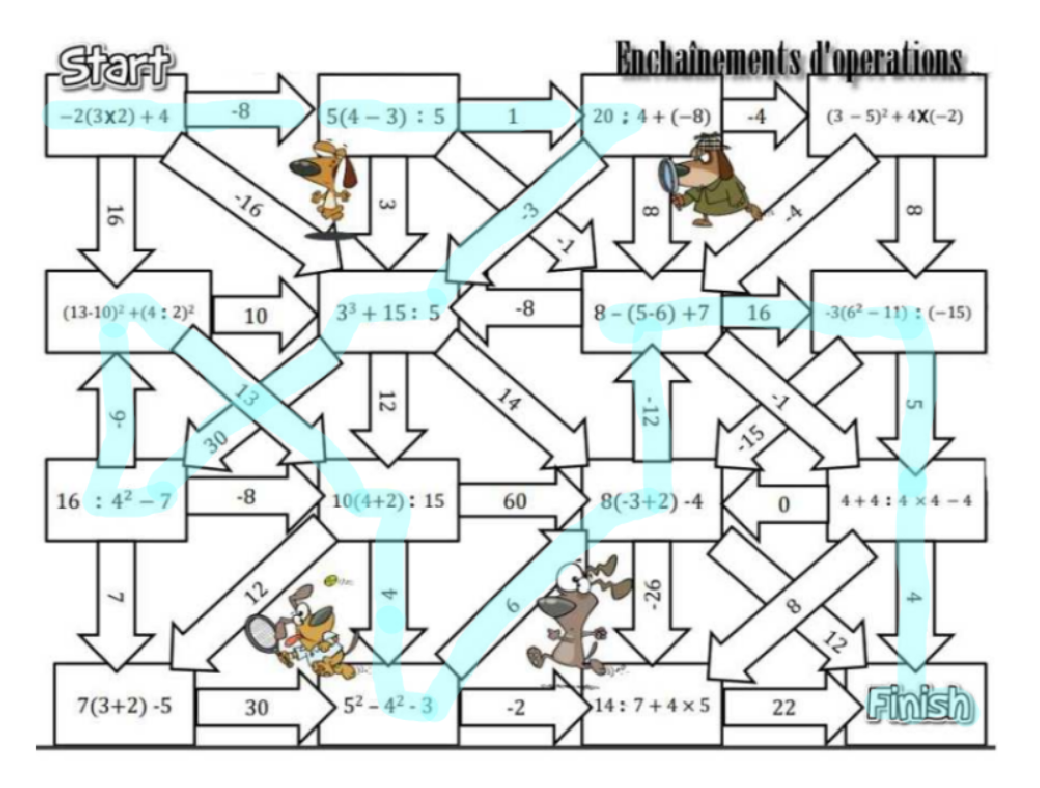
\includegraphics[scale=0.9]{labyrinthe.eps} \\

\vspace*{0.5cm}

\bmul{2}
\exo \\
Écrire les nombres suivants sous forme de puissance de 10. \\



\noindent 1 000 = \textcolor{red}{$10^{3}$}\\
100 000 000 = \textcolor{red}{$10^{8}$} \\
0,0000001 = \textcolor{red}{$10^{-7}$} \\
0,1 = \textcolor{red}{$10^{-1}$}\\
0,001 = \textcolor{red}{$10^{-3}$}\\
 

\columnbreak

\exo \\
Associer les écritures scientifiques avec les nombres auxquels elles correspondent. \\



\includegraphics[scale=0.6]{correctionpuissances.eps} 



\emul

\vspace*{0.5cm}

\exo \\
Écrire les nombres suivants à l'aide de l'écriture scientifique. \\

\bmul{3}

M = 7 890 \\

\textcolor{red}{$M = 7,89 \times 10^{3}$}\\







\columnbreak


$R = 0,67 \times 10^{-3}$\\

\textcolor{red}{$R = 6,7 \times 10^{-4}$}\\

\columnbreak

$L = 0,003 \times 10^{6}$\\

\textcolor{red}{$L = 3,0 \times 10^{3}$}\\


\emul
\vspace*{0.5cm}


\vspace*{0.5cm}
\exo \\
Voici les distances entre le soleil et les planètes du systèmes solaire :  

\renewcommand{\arraystretch}{1.5}

\begin{center}
\begin{tabular}{|c|c|}
\hline 
Vénus : 105 millions km &  Mercure : $58 \times 10^{6}$ km \\ 
\hline 
Mars : $2 250 \times 10^{5}$ km &  Terre : $15 \times 10^{7}$ km \\ 
\hline 
 Uranus : 2 880 millions km & Saturne : 1 425 000 000 km \\ 
\hline 
Jupiter : 780 000 000 km &  Neptune : $45 \times 10^{8}$ km \\ 
\hline 
\end{tabular}
\end{center}

 \textbf{Ranger ces distances par ordre croissant }(attention pour les comparer il faut les écrire à l'aide de l'écriture scientifique).\\

\color{red}

On commence par exprimer la distance de chaque planète en écriture scientifique :\\

\bmul{3}

$V = 1,05  \times 10^{8}$\\

$J = 7,8 \times 10^{8}$\\

$S = 1,425 \times 10^{9}$\\

\columnbreak

$Ma = 2,25 \times 10^{8}$\\

$Me = 5,8 \times 10^{7}$\\

$N = 4,5 \times 10^{9}$\\

\columnbreak

$U = 2,88 \times 10^{9}$\\

$T = 1,5 \times 10^{8}$\\

\emul



Dans l'ordre croissant, on obtient Mercure, Vénus, la Terre, Mars, Jupiter, Saturne, Uranus et Neptune.\\


\color{black}



\newpage
\end{document}
